\documentclass{article}

\begin{document}

\setlength{\parindent}{6ex}

\begin{figure}
    \centering
    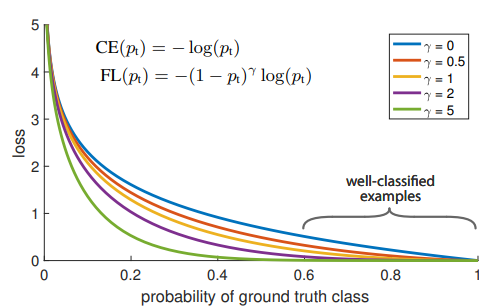
\includegraphics[width=0.75\textwidth]{focalloss}
    \caption{Focal Loss}
    \label{fig:focalloss1}
\end{figure}

\indent

In general, two-stage detectors have a better accuracy than one-stage 
detectors. The aim of this article is to find out why this is the case. 
Two-stage detectors are applied on a sparse set of candidate object 
locations. However, one-stage detectors are applied over dense sampling 
of possible object locations. Then, the obtained result is the 
foreground-background class imbalance in training of dense detectors.
The improved solution to this problem is called focal loss (Fig. 
\ref{fig:focalloss1}) which is introduced by this article. \par

Focal loss is the reshaped version of cross-entropy loss. The aim of 
this change in cross-entropy is to down-weights the loss calculated for 
well-classified examples. Thus, detector is trained on sparse set of 
hard examples. Also, class imbalance is handled by focal loss and 
sampling examples is not required since well-learned examples do not 
overwhelm loss during training. You can see the change in loss by looking 
figure \ref{fig:focalloss1}. When $\gamma$ equals to zero, focal loss is 
equivalent to cross-entropy loss. For higher values of $\gamma$, the 
convergence of loss values changes as in the figure \ref{fig:focalloss1}. 
The best-performing $\gamma$ value equals to two according to the article.

\begin{figure}
    \centering
    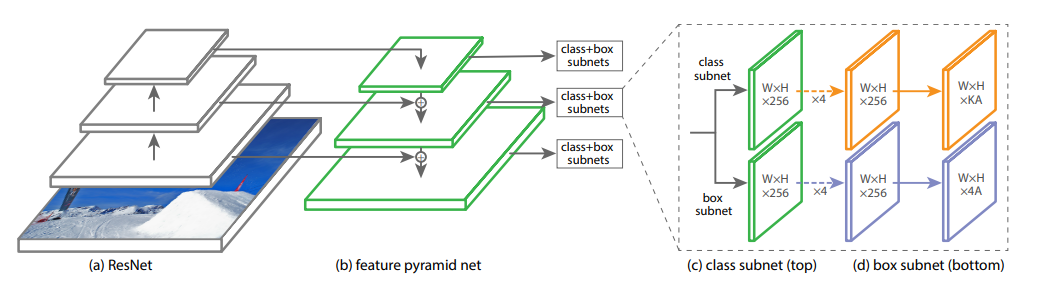
\includegraphics[width=\textwidth]{models/retinanet}
    \caption{Network of RetinaNet}
    \label{fig:retinanet1}
\end{figure}
\indent

RetinaNet is designed to show the effectiveness of Focal Loss. As you 
can see in figure \ref{fig:retinanet1}, RetinaNet uses ResNet as its 
backbone network and FPN to obtain a multi-scale convolutional feature 
pyramid. Then, two subnetworks are used to obtain detection results. 
One of them is used to classify anchor boxes to obtain classification of 
objects in anchor boxes and the other one is used to regress bounding 
boxes from anchors in which the aim is to obtain ground-truth bounding 
boxes.
\end{document}